\documentclass[tikz]{standalone}

\usetikzlibrary{arrows, shapes, positioning}

\begin{document}
    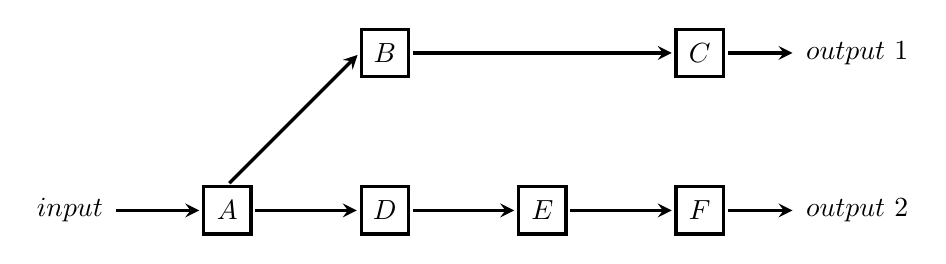
\begin{tikzpicture}[scale=4, >=stealth, node distance=2cm, shorten >=1pt, shorten <=1pt, minimum size=0.6cm, very thick]
        \node[] (data) {$input$};
        \node[rectangle, draw, right of=data] (A) {$A$};
        \node[rectangle, draw, right of=A] (D) {$D$};
        \node[rectangle, draw, above of=D] (B) {$B$};
        \node[rectangle, draw, right of=D] (E) {$E$};
        \node[rectangle, draw, right of=E] (F) {$F$};
        \node[rectangle, draw, above of=F] (C) {$C$};
        \node[right of=C] (output1) {$output\ 1$};
        \node[right of=F] (output2) {$output\ 2$};
        
        \draw[->] (data) -- (A);
        \draw[->] (A.north) -- (B.west);
        \draw[->] (B) -- (C);
        \draw[->] (A) -- (D);
        \draw[->] (D) -- (E);
        \draw[->] (E) -- (F);
        \draw[->] (F) -- (output2);
        \draw[->] (C) -- (output1);
    \end{tikzpicture}
\end{document}
